%%%%%%%%%%%%%%%%%%%%%%%%%%%%%%%%%%%%%%%%%%%%%%%%%%%%%%%%%%%%%%%%%%%%%%%%%%%%%%%%
%2345678901234567890123456789012345678901234567890123456789012345678901234567890
%        1         2         3         4         5         6         7         8

\documentclass[letterpaper, 10 pt, conference]{ieeeconf}  % Comment this line out if you need a4paper

%\documentclass[a4paper, 10pt, conference]{ieeeconf}      % Use this line for a4 paper

\IEEEoverridecommandlockouts                              % This command is only needed if
                                                          % you want to use the \thanks command

\overrideIEEEmargins                                      % Needed to meet printer requirements.

%In case you encounter the following error:
%Error 1010 The PDF file may be corrupt (unable to open PDF file) OR
%Error 1000 An error occurred while parsing a contents stream. Unable to analyze the PDF file.
%This is a known problem with pdfLaTeX conversion filter. The file cannot be opened with acrobat reader
%Please use one of the alternatives below to circumvent this error by uncommenting one or the other
%\pdfobjcompresslevel=0
%\pdfminorversion=4

% See the \addtolength command later in the file to balance the column lengths
% on the last page of the document

% The following packages can be found on http:\\www.ctan.org
\usepackage{graphics} % for pdf, bitmapped graphics files
\usepackage{epsfig} % for postscript graphics files
\usepackage{mathptmx} % assumes new font selection scheme installed
%\usepackage{times} % assumes new font selection scheme installed
\usepackage{amsmath} % assumes amsmath package installed
\usepackage{amssymb}  % assumes amsmath package installed
%\usepackage{algorithmicx}
%\usepackage[Algorithm,ruled]{algorithm}
%\usepackage{algpseudocode}
\usepackage{tabularx}
\usepackage{fancyhdr}
\usepackage{multirow}
\usepackage{color}
\usepackage[hyphens]{url}
\usepackage{breakurl}
%\usepackage{balance}
\usepackage{subcaption}
\usepackage{breqn}
\usepackage{algorithm2e}
\usepackage{dblfloatfix} 
\usepackage[export]{adjustbox}
\usepackage{tabulary,booktabs}

%\usepackage{verbatim}
%\usepackage{flushend}

\newcommand{\junk}[1]{}
\newcommand{\abs}[1]{\left| #1 \right|} %| |
\newcommand{\comment}[1]{\textcolor{red}{#1}}

\title{\LARGE \bf
%Autonomous Mobile Service Robots for Tending to Healthy Quarantined Individuals
Autonomous Pick and Place of Cylindrical Objects using Visual (RGB-D) and Tactile Sensing
}

\author{\IEEEauthorblockN{Alejandro Halpern Pastor$^{1}$
\thanks{$^{1}$ Department of Computer Science, University College London, Gower Street, WC1E 6BT, UK.}}
\and\IEEEauthorblockN{Andras Nagy$^{1}$\\}
\and\IEEEauthorblockN{Tim Andersson$^{1}$\\}
\and\IEEEauthorblockN{Xingjian Lu$^{1}$\\}}

\date{09 March 2021} %it will not be displayed

\begin{document}



\maketitle
\thispagestyle{fancy}
\pagestyle{plain}
\fancyhf{}
\rhead{13/04/2021}
\cfoot{\thepage}

\begin{abstract}
This paper demonstrates a methodology to enable a Emika Panda 7-DoF arm to pick and place a cylindrical object from the floor and in between 3 tables utilising RGB-D and bumper sensing. The cylinder pose is detected by performing filtering and SAC segmentation on the RGB-D point cloud, upon which MoveIt! motion planning is used to plan and the pick and place operation. The proposed methodology is implemented and tested within the RViz simulation environment, where it is shown to successfully perform its function.
\end{abstract}

% \newpage
\section{Introduction}\label{Sec:introduction}
%%%%%%%%%%%%%%%%%%%%%%%%%%%%%%%%%%%%%%%%%%%%%%%%%%%%%%%%%%%%%%%%%%%%%%%%
\subsection*{Objectives}
In this paper 2 pieces of software are developed, one to detect the pose of a cylinder using and RGB-D camera and a second one to pick and place said cylinder in between 3 target locations. Additionally, once the first grasp is initiated, only bumper sensing will be used to keep track of the location of the cylinder object.

%%%%%%%%%%%%%%%%%%%%%%%%%%%%%%%%%%%%%%%%%%%%%%%%%%%%%%%%%%%%%%%%%%%%%%%%
\subsection*{Problem Setup}
The robot used for the pick and place task will be a Franka Emika Panda 7-DoF manipulator. The manipulator is set-up in the RViz environment shown in Figure \ref{fig:setup}.

The manipulator is directly facing a wall and the target cylinder to be picked, which is resting on the floor. The manipulator is also surrounded by 3 tables, which will serve as the target locations for the cylinder placement. 

Each table has a bumper sensor at its center that will indicate to the robot whether the table is occupied or not. One of the tables contains a box object that will have to be re-positioned to make space for the cylinder should it be moved to the same table.

The RGB-D camera will be placed as shown by the frame in Figure \ref{fig:setup}, pointing towards the wall and cylinder object.

\begin{figure}[h]
    \centering
    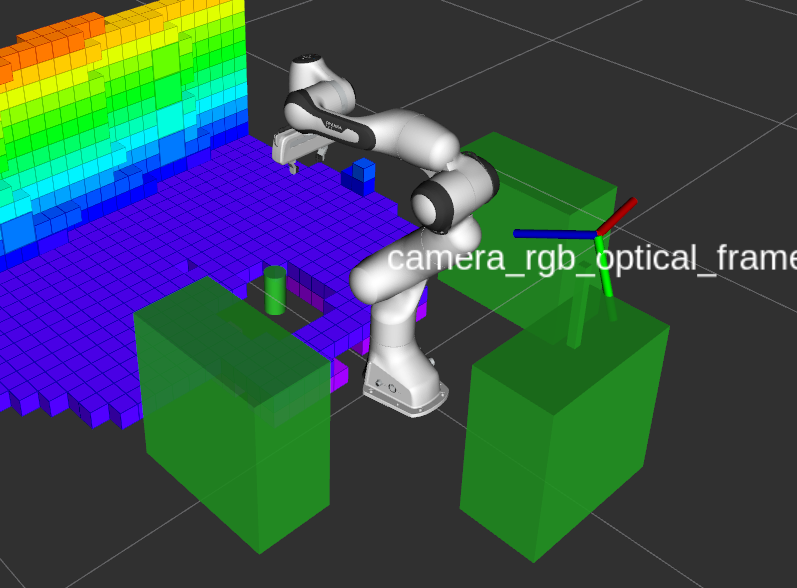
\includegraphics[width=8cm]{Images/Setup.png}
    \caption{RViz simulation environment setup. The voxel-grid indicates the floor and wall as perceived by the camera. MoveIt! collision objects are displayed in green.}
    \label{fig:setup}
\end{figure}

%%%%%%%%%%%%%%%%%%%%%%%%%%%%%%%%%%%%%%%%%%%%%%%%%%%%%%%%%%%%%%%%%%%%%%%%
\subsection*{Related Work}
The software used for cylinder detection makes use of the Random Sample Consensus (RANSAC) algorithm  \cite{RANSAC} to segment the RGB-D point cloud generated by the camera. Identifying (using RANSAC) the points of the point cloud that fit a cylindrical model, we are effectively removing the floor and wall from the point cloud. From those remaining points and the fitted model the cylinder's dimensions and pose can be ascertained. Both RANSAC and the point cloud management are implemented using the PCL library \cite{PCL}.

The robot path planning and control, the bumper sensors and the collision objects are implemented through the MoveIt! library \cite{moveit}.

% \newpage
\section{Methodology}\label{Sec:intro}
%%%%%%%%%%%%%%%%%%%%%%%%%%%%%%%%%%%%%%%%%%%%%%%%%%%%%%%%%%%%%%%%%%%%%%%%
\subsection*{Visual}\label{Sec:methvis}
In order to extract the pose of the target cylinder from the RGB-D point cloud generated by the camera, it is necessary to separate the points corresponding to the cylinder from the rest of the points. Knowing that the cylinder is the only cylindrical object in the point cloud, RANSAC can be used to identify the points corresponding to an infinite cylindrical model based on their position and surface normals. From the fitted model the cylinder pose and radius can be extracted. The cylinder height and centre point can then be found using the lowest and highest points of the cylinder and the camera pose.

However, the point cloud's large number of data-points can slow down computation of the cylinder pose. To fix this, two filters where implemented. The first one was a downsampling filter, which applied a voxel grid of a specified size over the entire point cloud and merged the multiple points in each voxel into a single, averaged one. The second was a passthrough filter, which involved removing all points outside of the approximate area the cylinder was expected to lie in. These two approaches removed the number of points in the pointcloud and sped up the RANSAC computation, at the cost of a lower resolution (from the downsampling filter) leading to a lower accuracy in the cylinder pose.
%%%%%%%%%%%%%%%%%%%%%%%%%%%%%%%%%%%%%%%%%%%%%%%%%%%%%%%%%%%%%%%%%%%%%%%%
\subsection*{Motion}
In order to perform motion planning for this task the MoveIt ROS library is used. The cylinder pose is extracted using the methods described in the section above, and then MoveIt is used to perform inverse kinematics to find the robot configurations necessary to approach, grasp, retreat, and place the cylinder and the cuboid object.

The version of MoveIt used for this task uses iterative inverse kinematics (IIK) rather than any closed form solutions. This is less than ideal due to the fact IIK is much less consistent than closed form solutions and can sometimes not come up with any solution at all. IIK can also be very slow depending on the current manipulator configuration and the desired one. The cuboid pose and the pose of the tables are acquired from the MoveIt simulation. 

% \newpage
\section{Experiments}\label{Sec:experiments}
%%%%%%%%%%%%%%%%%%%%%%%%%%%%%%%%%%%%%%%%%%%%%%%%%%%%%%%%%%%%%%%%%%%%%%%%
A simulation environment was created in RViz in order to test the aforementioned methodologies.
\subsection*{Visual}
The goal of question 1 is to improve upon the existing segmentation algorithm and to make it execute faster. As mentioned in section \ref{Sec:methvis}, three types of filters are tested and analysed against their effects on execution time and segmentation accuracy are also compared with the case where no filter is applied (NON). For question 1.1, VoxelGrid (VG) and StatisticalOutlierRemoval (SOR) are used. For question 1.2, a PassThrough filter (PT) is used based on the question description. The resulting point cloud can be found in fig. \ref{fig:t1}. 

\begin{figure}[h!]
    \centering
    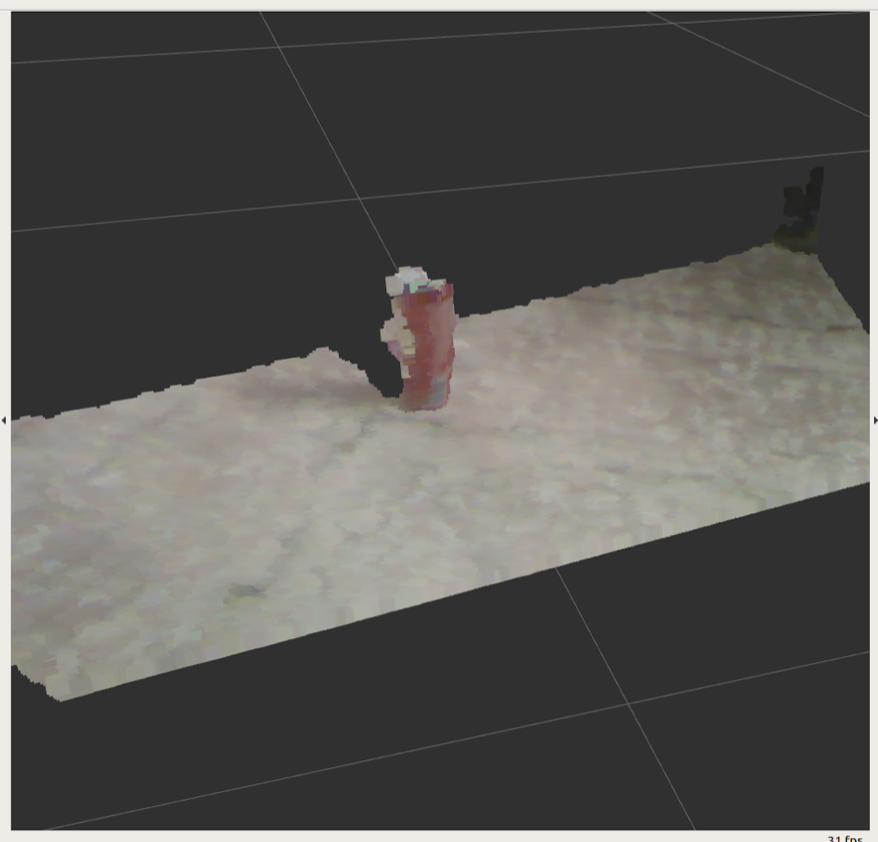
\includegraphics[width=.2\textwidth]{Images/non.png}
    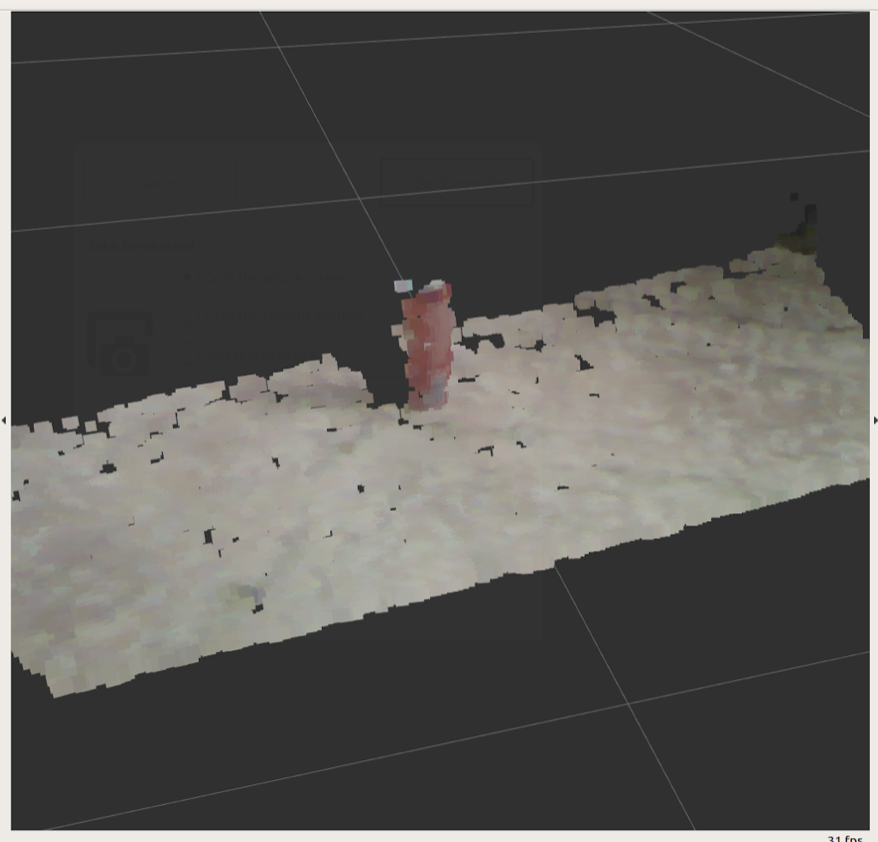
\includegraphics[width=.2\textwidth]{Images/1.1.png}
    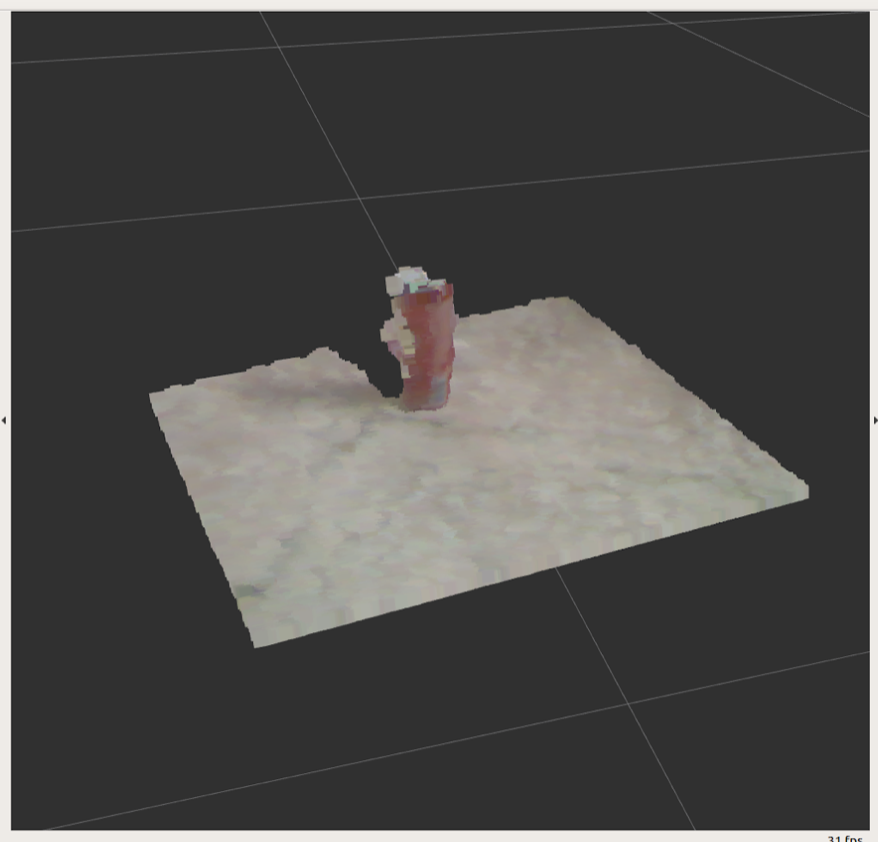
\includegraphics[width=.2\textwidth]{Images/1.2.png}
    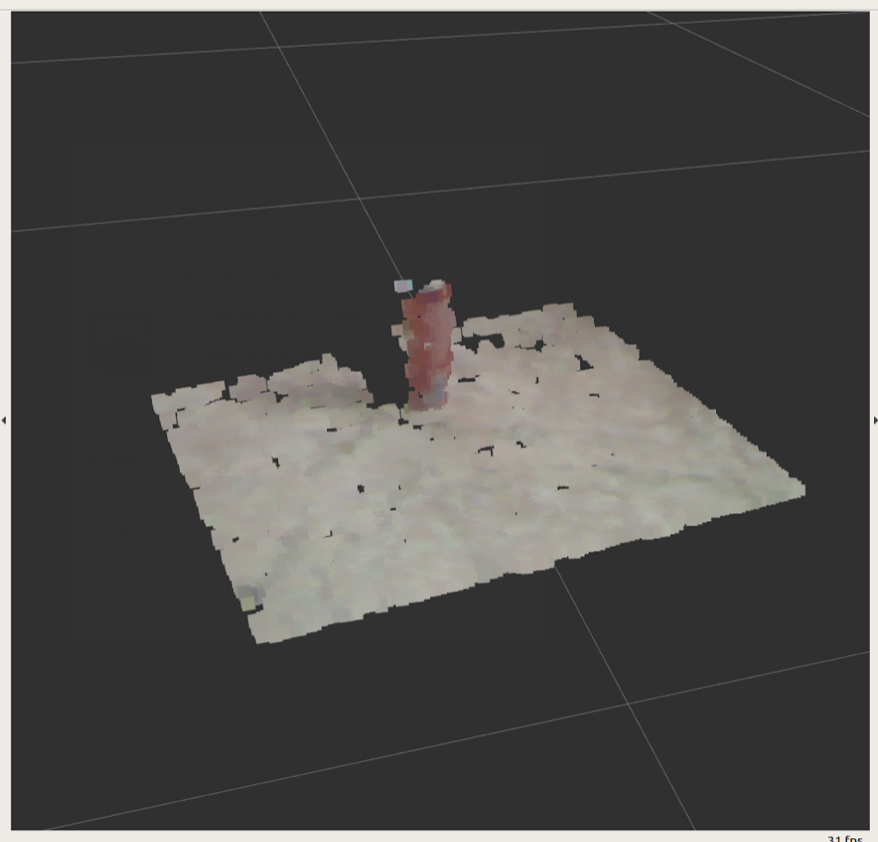
\includegraphics[width=.2\textwidth]{Images/both.png}
    \caption{Filtered PointCloud; top left: no filter; top right: with filters in q1.1; bottom left: with filters in q1.2; bottom right: with filters in both q1.1 and q1.2}
    \label{fig:t1}
\end{figure}

\subsubsection*{Time}
The time consumption of applying filter, segmentation and the total of the two are recorded for different combinations of filters. The following table shows the average time for each filtering function over a randomly-chosen 10 consecutive seconds.
\begin{table}[h!]
\begin{center}
 \begin{tabular}{|c c c c|}
 \hline 
 time(ms) & filtering &  segmentation & total \\
 \hline 
 NON &  24.9 &  634.3 &  659.2\\
 \hline 
 VG &  43.4 &  174.8 &  218.2\\
 \hline 
 SOR &  411.6&  459.1 &  870.7\\
 \hline 
 VG+SOR &  146.2 &  138.7 &  284.9 \\
 \hline 
 PT &  43.1 &  361.2&  404.3 \\
 \hline 
 VG+SOR+PT &  146.1 &  64.4 &   210.5\\
  \hline 
 VG+PT &  48.6 &  92.9 &  141.5 \\
 \hline
\end{tabular}
\end{center}
\caption{time performance of different filtering algorithms}
\label{table:1}
\end{table}

From here we can conclude the following:
\begin{itemize}
    \item in terms of improvement of segmentation performance, the combination of all three filter works the best with the result being 10.15\% of the original time.
    \item in terms of improvement of total performance, counting filtering and segmentation, the combination of VG and PT works the best, with the result being 21.47\% of the original time.
    \item there's a trade-off between the improvement of segmentation performance and using filtering algorithms. More complicated filtering could results in better segmentation performance but meanwhile longer filtering time. 
    \item because the goal of the coursework is to improve the segmentation performance, both SOR and VG are included in question 1.1. 
\end{itemize}

\subsubsection*{Accuracy}
To assess the accuracy of the segmentation. The resulting cylinder pose and size after applying each filter combination are compared against the pose and size when no filter is applied. The following table shows the average results for each filtering function over a randomly-chosen 10 consecutive seconds.

\begin{table}[h!]
\begin{center}
 \begin{tabular}{|c c c c c c|}
 \hline 
 meters & radius &  height & centre x & centre y & centre z \\
 \hline 
 NON &  0.030 &  0.120 & -0.052 & 0.157 &  0.934 \\
 \hline 
 VG &  0.029 &  0.119 &  -0.050 & 0.156 & 0.933\\
 \hline 
 SOR &   0.028 & 0.121 & -0.053 & 0.157 & 0.934 \\
 \hline 
 VG+SOR & 0.025  & 0.121 & -0.055 &0.154 & 0.935\\
 \hline 
 PT &  0.028 & 0.121 & -0.049 & 0.158 &  0.933\\
 \hline 
 VG+SOR+PT &  0.024  &  0.119 & -0.058 & 0.155 & 0.935 \\
  \hline 
 VG+PT &   0.032 & 0.119 & -0.050 & 0.156 & 0.933 \\
 \hline
\end{tabular}
\end{center}
\caption{resulting cylinder position and size of different filtering algorithms}
\label{table:1}
\end{table}

Although we do not have a strict metric for comparing accuracy in terms of the size and position of the resulting cylinder, by roughly looking at the numbers we can see that VG works best when estimating the size of the cylinder and SOR works best when estimating the position of the cylinder. The more complex the filtering algorithms are, the more inaccurate the estimation of cylinder is. Two of the best performing filter combination in terms of time complexity performs relatively poorly here. 

\subsubsection{Conclusion}

From the comparison between different filtering algorithms on their time and accuracy performance, we can see a clear trade-off between the two. More complex combination of filters could result in faster segmentation but less accuracy result and vice versa. 

%%%%%%%%%%%%%%%%%%%%%%%%%%%%%%%%%%%%%%%%%%%%%%%%%%%%%%%%%%%%%%%%%%%%%%%%
\subsection*{Motion}
After the cylindrical object is grasped, only information is coming from the bumper sensors, no further motion capture system is used. In order test the performance of the bumper sensors and the pick and place process several experiments were made where the motion was controlled by the '1', '2' and '3' keys. The experiments of the bumpers can be said successful if they change accordingly and immediately when an object is put or lifted up from the table, which was examined by checking the published Boolean values on the appropriate topics. The performance of the grasp and transportation of the objects is evaluated by executing several different combinations of pick and place tasks and the number of successful attempts are counted. The Franka Emika Panda robotic arm can be seen during a pick and place task on Figure \ref{fig:cylindrical grasp}.


First, the pick and place process of the cylindrical object was tested. By pressing one, the cylindrical object was grasped by a top grasped and placed on the first table.    

\begin{figure}[h]
    \centering
    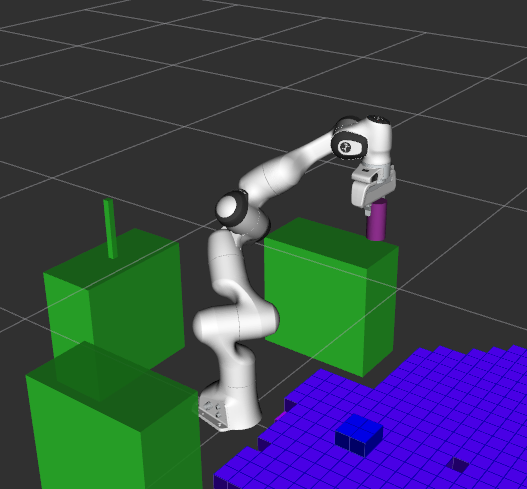
\includegraphics[width=8cm]{Images/cylindrical_grasp.png}
    \caption{A successful top grasp of the cylindrical object, purple highlights that the object is being grasped}
    \label{fig:cylindrical grasp}
\end{figure}

Then, a more complex process was tested. By pressing '2', the robot had to identify from the bumper sensors that table two is occupied; therefore, the robotic arm first needed to place the cubic object to a free table and then, the cylindrical object was moved. Figure \ref{fig:task 2} shows the scene after the aforementioned task was finished.

\begin{figure}[h]
    \centering
    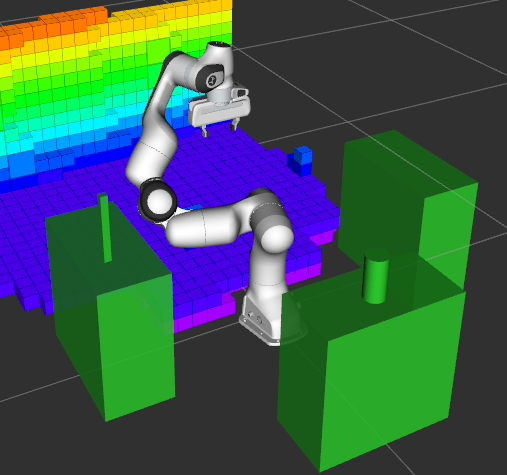
\includegraphics[width=8cm]{Images/task2.png}
    \caption{A Finished, successful task 2}
    \label{fig:task 2}
\end{figure}

Next, further experiments were made; for instance, the transportation of the cylindrical object to the third table and the placement of the cylindrical object to different tables when it is off the ground were executed. During all the attempts, the relevant bumper topics were examined. It can be said that the sensors work properly and detect the changes immediately. 

Overall, the experiments were , and it can be said that the implemented method fulfils the requirements. 
% \newpage
\section{Conclusions and Future Work}\label{Sec:conclusions}
%%%%%%%%%%%%%%%%%%%%%%%%%%%%%%%%%%%%%%%%%%%%%%%%%%%%%%%%%%%%%%%%%%%%%%%%
Section \ref{Sec:experiments} shows that the applied methodology fulfilled the cylinder detection and pick and place requirements. 

In terms of cylinder detection, it successfully used RANSAC to extract the cylinder pose from the RGB-D data, as shown in Table 1. Additionally, the implementation of the point cloud filters successfully decreased the cylinder segmentation time to 21.47 \% of the original time. Furthermore, the bumper sensors successfully kept track of both the cylinder and cuboid objects when they were located in the centre of any table.

In terms of pick and place, the implemented methods were demonstrated to be able to pick and place the cylinder into any of the 3 tables, removing the cuboid object beforehand if it was in the way.

The following future research avenues are proposed:

\begin{itemize}
    \item Replace all sensing with a wrist mounted RGB-D camera, that allows the robot to map its environment and keep track of the position of all objects without the need for bumper sensors in the tables.
    
    \item Use a more sophisticated methodology for grasp detection that allows the robot to grasp irregularly shaped objects.
    
    \item Remove the need to pick and place objects only from the centre of tables, thus allowing both the cylindrical and cuboid objects to be placed in the same table hence accelerating workflow.
    
\end{itemize}

\newpage

\bibliographystyle{IEEEtran}
\bibliography{references}
\end{document}